\documentclass[a4paper,twoside,11pt]{article}
\usepackage{a4wide,graphicx,fancyhdr,amsmath,amssymb,placeins}
\usepackage{listings}
\usepackage{color}
\usepackage{enumitem}
\usepackage{amsmath}
\usepackage{textcomp}
\usepackage{caption,subcaption}
\usepackage{placeins}

%----------------------- Macros and Definitions --------------------------

\setlength\headheight{20pt}
\addtolength\topmargin{-10pt}
\addtolength\footskip{20pt}

\newcommand{\N}{\mathbb{N}}
\newcommand{\ch}{\mathcal{CH}}
\newcommand{\cpp}{{\tt C++} }

\newcommand{\solution}[1][todo]{\noindent{\bf Solution to Exercise #1:}}
\newcommand{\todo}[1]{{\Large\sc\textcolor{red}{#1}}}

\renewcommand{\lstlistingname}{Codeblock}
\captionsetup[lstlisting]{font={small,tt}}

\fancypagestyle{plain}{%
\fancyhf{}
\fancyhead[LO,RE]{\sffamily\bfseries\large technische universiteit eindhoven}
\fancyhead[RO,LE]{\sffamily\bfseries\large 2IW02 RTSD}
\fancyfoot[LO,RE]{\sffamily\bfseries\large department of mathematics and computer science}
\fancyfoot[RO,LE]{\sffamily\bfseries\thepage}
\renewcommand{\headrulewidth}{0pt}
\renewcommand{\footrulewidth}{0pt}
}

\pagestyle{fancy}
\fancyhf{}
\fancyhead[RO,LE]{\sffamily\bfseries\large technische universiteit eindhoven}
\fancyhead[LO,RE]{\sffamily\bfseries\large 2IW02 RTSD}
\fancyfoot[LO,RE]{\sffamily\bfseries\large department of mathematics and computer science}
\fancyfoot[RO,LE]{\sffamily\bfseries\thepage}
\renewcommand{\headrulewidth}{1pt}
\renewcommand{\footrulewidth}{0pt}

%-------------------------------- Title ----------------------------------

\title{\vspace{-\baselineskip}\sffamily\bfseries Exercise 2}
\author{
	Rick Veens \qquad Studentno: 0912292\\
	\texttt{r.veens@student.tue.nl}
	\and
	Huib Donkers \qquad Studentno: 0769015\\
	\texttt{h.t.donkers@student.tue.nl}
}

\date{\today}

\definecolor{listinggray}{gray}{0.9}
\definecolor{lbcolor}{rgb}{0.9,0.9,0.9}
\lstset{
backgroundcolor=\color{lbcolor},
    tabsize=4,    
%   rulecolor=,
    language=[GNU]C++,
        basicstyle=\scriptsize,
        upquote=true,
        aboveskip={1.5\baselineskip},
        columns=fixed,
        showstringspaces=false,
        extendedchars=false,
        breaklines=true,
        prebreak = \raisebox{0ex}[0ex][0ex]{\ensuremath{\hookleftarrow}},
        frame=single,
        numbers=left,
        showtabs=false,
        showspaces=false,
        showstringspaces=false,
        identifierstyle=\ttfamily,
        keywordstyle=\color[rgb]{0,0,1},
        commentstyle=\color[rgb]{0.026,0.112,0.095},
        stringstyle=\color[rgb]{0.627,0.126,0.941},
        numberstyle=\color[rgb]{0.205, 0.142, 0.73},
%        \lstdefinestyle{C++}{language=C++,style=numbers}’.
}

% geen stomme indents bij \par
\setlength{\parindent}{0cm}
\setlength{\parskip}{1em}

%--------------------------------- Text ----------------------------------

\begin{document}
\maketitle

\section{Timers}
\subsection{Model}
The model is shown in figure~\ref{fig:timermodel}, and code used for the first two tests in codeblock~\ref{code:timer}. The improved code used for the third test is shown in codeblock~\ref{code:timer2}. We used \texttt{octave} to parse the output as csv and perform some statistical analysis.

\begin{lstlisting}[caption=Pcode::execute, label=code:timer, language=C++]
void Pcode::execute()
{
  // protected region execute code on begin
	static struct timespec t1;


	struct timespec t2;
	struct timespec res;

	clock_gettime(CLOCK_REALTIME, &t2);
	clock_getres(CLOCK_REALTIME, &res);
	//long int elapsedTime = (t2.tv_usec - t1.tv_usec);

	printf("%ld.%.9ld, %ld.%.9ld, %ld.%.9ld\n", res.tv_sec, res.tv_nsec, t2.tv_sec, t2.tv_nsec, t1.tv_sec, t1.tv_nsec);

	t1 = t2;

	// protected region execute code end
}
\end{lstlisting}
\begin{lstlisting}[caption=Pcode::execute (improved), label=code:timer2, language=C++]
void Pcode::execute()
{
  // protected region execute code on begin
	static struct timespec t1;
	static uint64_t clockcycle;

	struct timespec t2;
	struct timespec res;
	uint64_t currentcycle = ClockCycles();

	clock_gettime(CLOCK_REALTIME, &t2);
	clock_getres(CLOCK_REALTIME, &res);
	int64_t dcycle= currentcycle-clockcycle;
	uint64_t cps = SYSPAGE_ENTRY(qtime)->cycles_per_sec;

	if(currentcycle > clockcycle)
		printf("%lld, %lld, %lld, %ld.%.9ld, %ld.%.9ld, %ld.%.9ld\n", currentcycle, clockcycle, cps, res.tv_sec, res.tv_nsec, t2.tv_sec, t2.tv_nsec, t1.tv_sec, t1.tv_nsec);

	t1 = t2;
	clockcycle = currentcycle;

	// protected region execute code end
}
\end{lstlisting}

\begin{figure}
 \centering
 \begin{subfigure}{\textwidth}
  \centering
  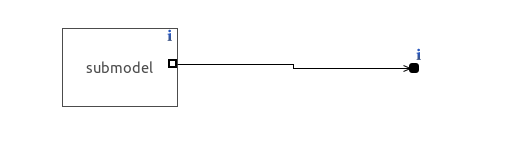
\includegraphics[width=0.8\textwidth]{./img/timer-mainmodel.png}
  \caption{Main model.}
 \end{subfigure}
 \begin{subfigure}{\textwidth}
  \centering
  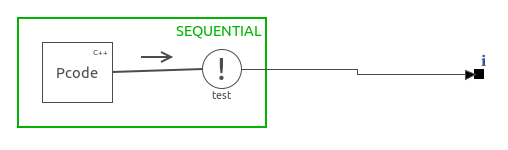
\includegraphics[width=0.8\textwidth]{./img/timer-submodel.png}
  \caption{submodel}
 \end{subfigure}
 \caption{Model used for testing the timer}
 \label{fig:timermodel}
\end{figure}

\FloatBarrier
\subsection{Questions} \label{sec:1_4}
\begin{enumerate}
 \item Measured over $1522$ intervals, the variation is $3.667 \cdot 10^{-8}$ s$^2$ or $0.03667$ ms$^2$. Since the clock resolution of QNX in virtual box ($0.000999848$ s) is so much larger than the observed variation, our measurements are not accurate enough to result in a variation that is representative for the actual variation. With a clock resolution of $0.000999848$ s, and a timer that ticks every $0.250000000$ s without jitter, we expect $\lceil 0.25/0.000999848 \rceil - 0.25/0.000999848 = 96.2\%$ of the measurements to be $\lfloor 0.25/0.000999848 \rfloor \cdot 0.000999848 = 0.249962$ s, and the other $3.8\%$ to be $\lceil 0.25/0.000999848 \rceil \cdot 0.000999848 = 0.250962$ s. In $1522$ measurements we found $96.2\%$ of the intervals to be $0.249962$ s and $3.8\%$ $0.250962$ s. Therefore, our measurements do not provide evidence of jitter.
 
 Up to a jitter bounded by $0.250000 - 0.249962 = 0.00038$ s $= 380$ $\mu$s, we would still expect the same results. For larger jitter, we would expect to occasionally measure intervals of $0.248962$ s. So we can strengthen our claim: our measurements do not provide evidence of jitter larger than $380$ $\mu$s.
 
 We performed a second series of measurements, this time with the timer interval set to $0.249962$, an exact multiple of the clock resolution. We measured $1967$ intervals. With this configuration, we are likely to pick up on a variation larger than $(0.000999848/1967 \cdot 10^6)^2 \approx 0.258$ $\mu$s$^2$.
 
 Results of the second test is shown in figure~\ref{fig:interval-jitter}. This shows that there is indeed jitter. The variation of our measurements is $0.06$ ms$^2$.
 
 For a third test we used a method of timing with a resolution that is much higher: \texttt{ClockCycles()} from \texttt{sys/neutrino.h}. We can retrieve the number of clock cycles per second, so we can deduce how much time has passed from the number of clock cycles that have passed. We measured $3339$ intervals using this method. The distribution of intervals is shown in figure~\ref{fig:interval-jitter2}. We can clearly see how the jitter behaves. It is still distributed somewhat discretely, but smaller deviations are now clearly shown. In this test the variation of the measurements is $0.078$ ms$^2$.
 
 \item This jitter is the result of simulating a real time OS in an environment that is not real time. Since the host OS decided when the virtual OS can run, and the host OS cannot guarantee to meet real time requirements, the virtual OS is unable to meet those requirements either.
 
 \item We observe from figure~\ref{fig:interval-jitter} that the timer tick is occasionally delayed by more than $1$ ms. Such a delay is not acceptable in many real time applications. What is worse, we have no guarantee that the delay is bounded. This could be catastrophic for an Anti-lock Brake System, or Autopilot.
 
 \item No. Our virtual machines run on a non real time OS (GNU/Linux), so it can happen that the host OS is very busy with tasks that have a higher priority than the virtual machines, postponing execution of the real time OS unboundedly, disabling QNX to meet its real time requirements.
 
\end{enumerate}

\begin{figure}
 \centering
 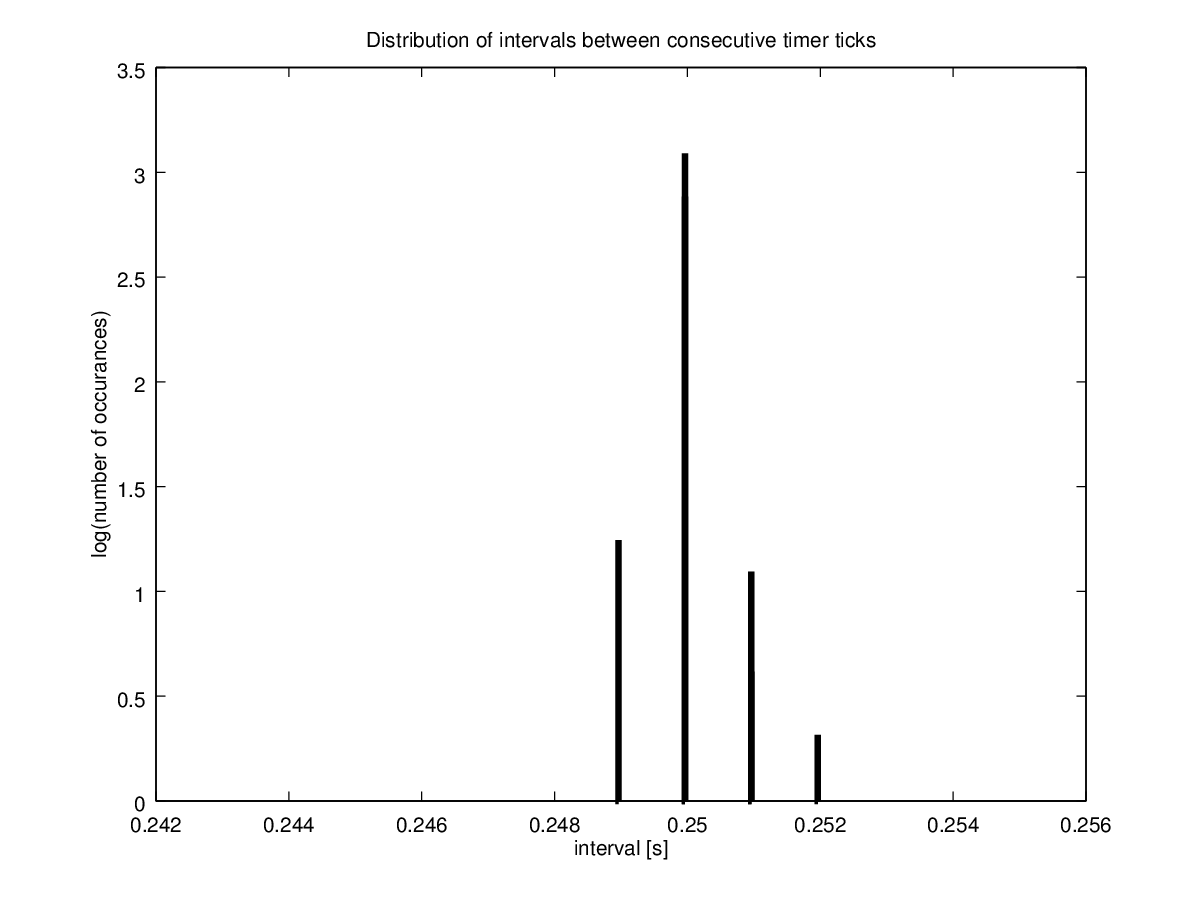
\includegraphics[width=0.8\textwidth]{./img/interval-jitter.png}
 \caption{Distribution of intervals in the second test.}
 \label{fig:interval-jitter}
\end{figure}
\begin{figure}
 \centering
 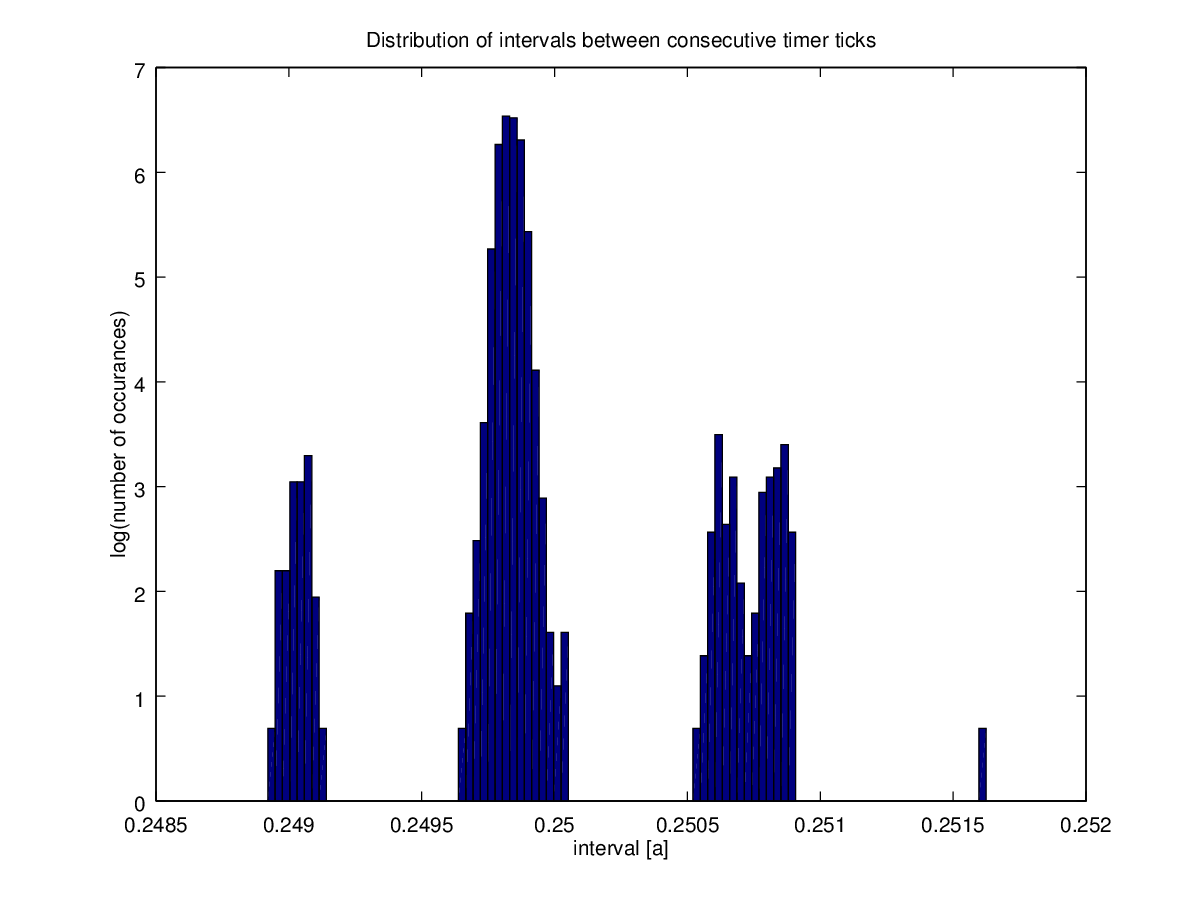
\includegraphics[width=0.8\textwidth]{./img/interval-jitter2.png}
 \caption{Distribution of intervals in the third test.}
 \label{fig:interval-jitter2}
\end{figure}

\FloatBarrier
\subsection{Validation}
We further extended the code measuring the intervals to send an alternating signal to an output pin (see codeblock~\ref{code:timer3}). The signal switches from high to low, or form low to high at each timer tick, producing a square wave of which we can measure the period using an oscilloscope.

\begin{lstlisting}[caption=Pcode::execute (extended), label=code:timer3, language=C++]
void Pcode::execute()
{
  // protected region execute code on begin
	static struct timespec t1;
	static uint64_t clockcycle;

	if (oc)
		oc = 0;
	else
		oc = 1;

	//printf("oc: %d\n", oc);

	struct timespec t2;
	struct timespec res;
	uint64_t currentcycle = ClockCycles();

	clock_gettime(CLOCK_REALTIME, &t2);
	clock_getres(CLOCK_REALTIME, &res);
	int64_t dcycle= currentcycle-clockcycle;
	uint64_t cps = SYSPAGE_ENTRY(qtime)->cycles_per_sec;

	if(currentcycle > clockcycle)
		printf("%lld, %lld, %lld, %ld.%.9ld, %ld.%.9ld, %ld.%.9ld\n", currentcycle, clockcycle, cps, res.tv_sec, res.tv_nsec, t2.tv_sec, t2.tv_nsec, t1.tv_sec, t1.tv_nsec);

	t1 = t2;
	clockcycle = currentcycle;

	// protected region execute code end
}
\end{lstlisting}

\subsection{Questions}
\begin{enumerate}
 \item Using the oscilloscope has the obvious disadvantages: it requires the availability of the oscilloscope, and an output pin. This output pin is not (easily) available for our dry-runs in a virtual machine. An additional disadvantage is that the supplied oscilloscope did not appear to have a function to measure a series of intervals easily. Only one measurement was shown on screen, updating frequently, making it very hard to generate a list of 1000-3000 measurements for an accurate assessment of the jitter like we did with the software method.
 
 The software method uses the same timing hardware to both produce the timer ticks, as to measure the intervals. This method only accurately measures the timer intervals, if the timing hardware is reliable.
 \item We ran two tests in the lab, one with a frequency of 4 Hz, and one with a frequency of 100 Hz. The readings from the oscilloscope seemed to agree with the measurements using the number of clockcycles, showing a period of 500.0 ms, sometimes 501.0 or 499.0 in the first run, and a period of 20.0 ms during the second run. We measured $758$ and $936$ intervals for 4 Hz and 100Hz respectively, using the number of clock cycles. Distribution of these measurements are shown in figure~\ref{fig:interval-jitter-rt} and figure~\ref{fig:interval-jitter-rt2}. Variation of these measurements are $0.053$ ms$^2$ and $0.0011$ ms$^2$ respectively. We see from the distribution that the test with 4 Hz resulted in two narrow peaks. We don't have an explanation for this, but clearly observe that the variation is a lot less than when using the virtual machine, more so than the actual variation of $0.053$ ms$^2$ would suggest.
 
 \item Not completely. We cannot explain that a small, though significant, amount of timer ticks is delayed by $1$ ms. We do expect this kind of behaviour on non real time systems, but not on a real time system. If we look at figure~\ref{fig:interval-jitter-rt2}, we see the timer behave according to theory: often right on time, occasionally slightly off, but always within a tight timeframe. When we compare figure~\ref{fig:interval-jitter-rt} and \ref{fig:interval-jitter2}, we see a similar improvement. The peaks become narrower, signalling that the timeframe is smaller. However we are unable to explain the presence of multiple of these peaks.
\end{enumerate}

\begin{figure}
 \centering
 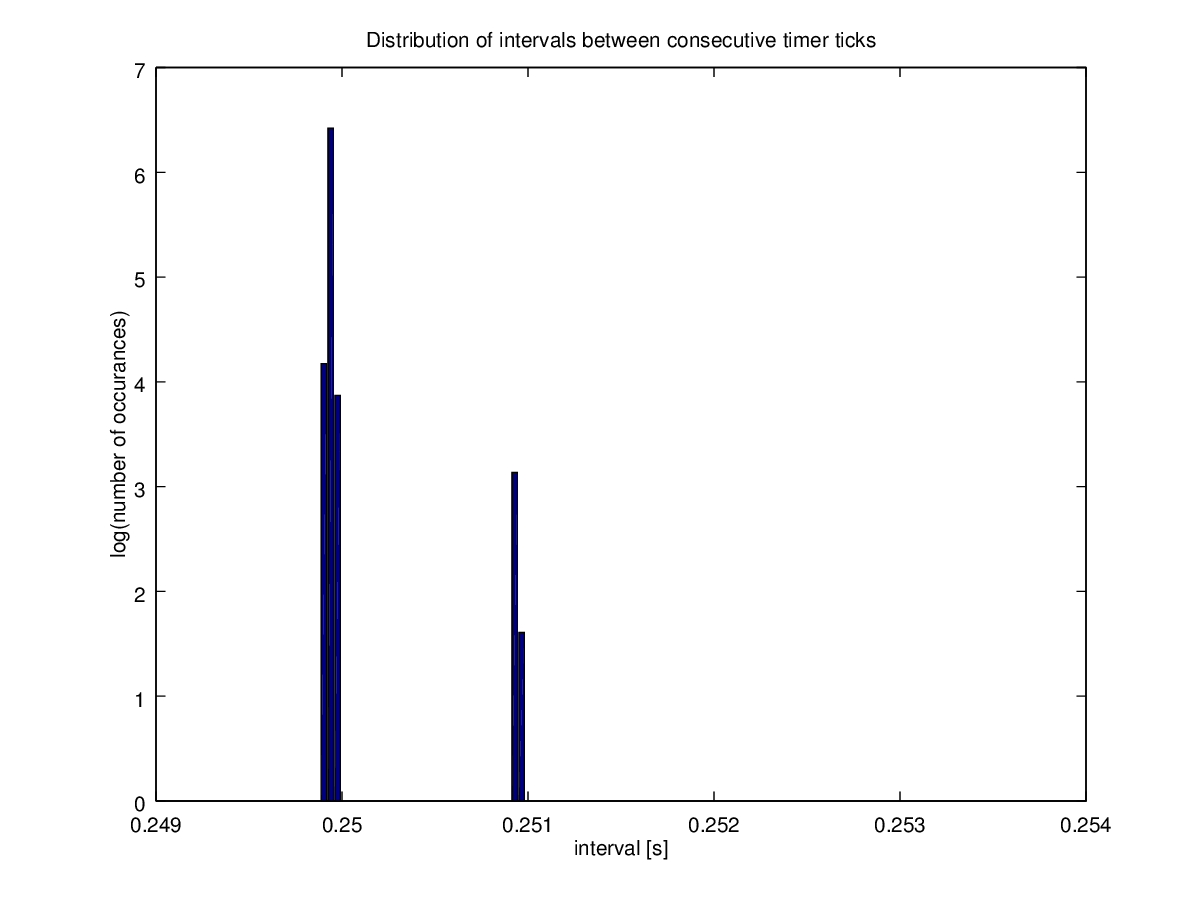
\includegraphics[width=0.8\textwidth]{./img/interval-jitter-rt.png}
 \caption{Distribution of intervals in the lab, with the timer set to 4 Hz.}
 \label{fig:interval-jitter-rt}
\end{figure}
\begin{figure}
 \centering
 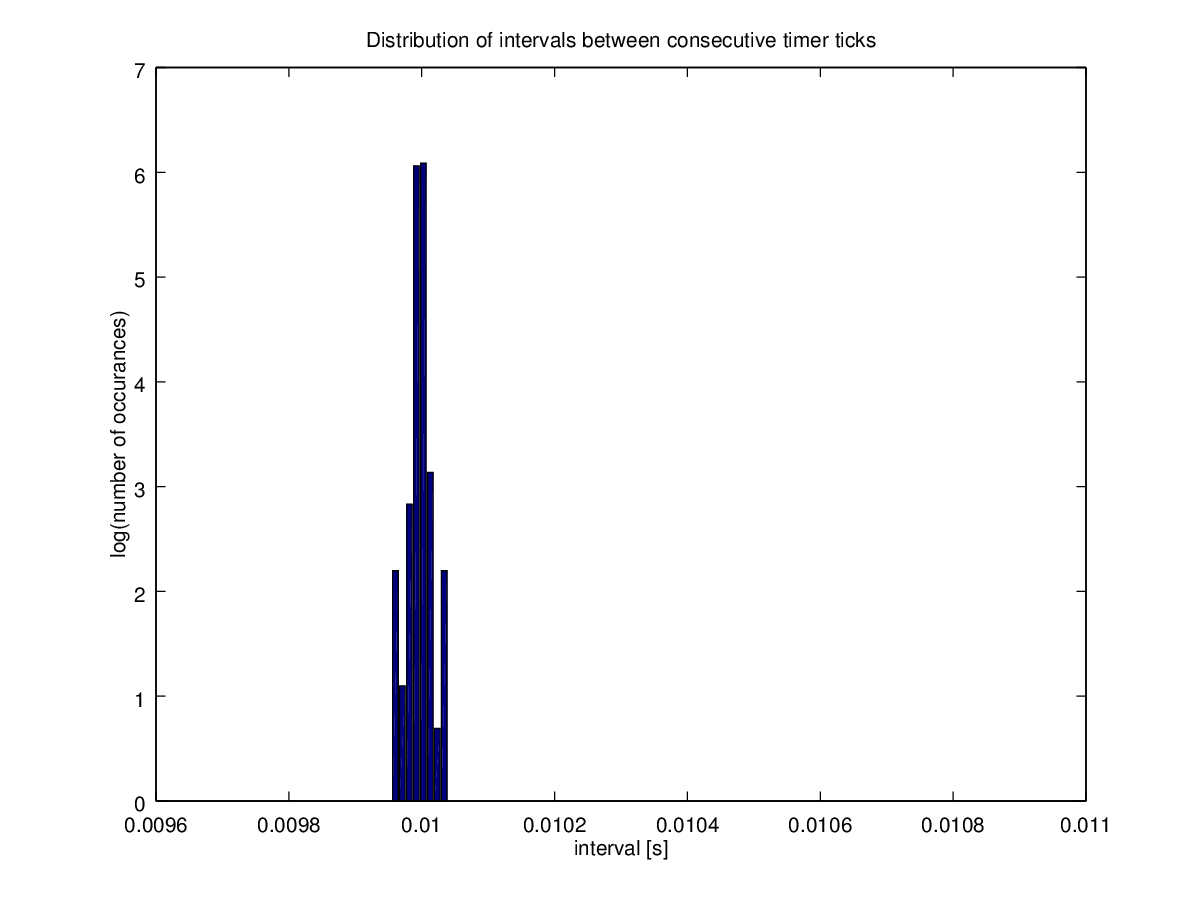
\includegraphics[width=0.8\textwidth]{./img/interval-jitter-rt2.png}
 \caption{Distribution of intervals in the lab, with the timer set to 100 Hz.}
 \label{fig:interval-jitter-rt2}
\end{figure}

\FloatBarrier
\section{JIWYIO Linkdrivers}
\subsection{JIWYIO driver components}
We made the two models suggested in the exercise description.
\subsubsection{PWMTester}
We tested writing some values to the simulated port first, see codeblock~\ref{code:pwmex}.
After that we made a function to convert from \texttt{int16\_t} to \texttt{uint16\_t} by using bit operations. However, we later found that this convert function could be replaced by a simple 
cast from \texttt{int16\_t} to \texttt{uint16\_t}, see codeblock~\ref{code:pwmcon}. Additionally, we made sure that any non-zero value would map to a value outside the deadzone of the motor.

At first we understood that the value JIWY outputs for engine steering would be a real between $-512$ and $512$. So we made a normalise function mapping this range to the range $[-1, 1]$.

\begin{lstlisting}[caption=Pcode::execute, label=code:pwmex, language=C++]
void Pcode::execute()
{
  // protected region execute code on begin
	static double t = 1.0;

	//t = -32768; // fast reverse
	//t = 32767; // fast forward
	//t = 32768; // stop
	//t = -1000; // deadzone?

	//this->test = (uint16_t) t;

	this->test = convert(normalise(t));
	printf("%lf, %lf, %d \n", t, normalise(t), convert(normalise(t)));
	//t+= 6.28318;
	while(t>512)
		t-= 1024;

  // protected region execute code end
}
\end{lstlisting}
\begin{lstlisting}[caption=Pcode::convert, label=code:pwmcon, language=C++]
uint16_t Pcode::convert(double f)
{
	int16_t deadzone = 2200;

	int16_t n = f*(32768-deadzone);
	if(n>0)
		n += deadzone;
	else if(n<0)
		n -= deadzone;

	if(n>=0 && n<32768)
		return n;
	else if(n >= -32768 && n<0)
	{
		return (uint16_t)n;
	}
	else
		return 0;
}
\end{lstlisting}
\begin{lstlisting}[caption=Pcode::normalise, label=code:pwmnor, language=C++]
double Pcode::normalise(double n)
{
	// linear conversion assumed
	double min=-512, max=512;

	// normalise to [-1,1]
	n-= min;
	n/= max - min;
	n*= 2;
	n-= 1;

	return n;

	/*
	// scale to int16_t
	if(n=1)
		return 32767;
	else
		return n*32768;
	//*/
}
\end{lstlisting}
\subsubsection{EncoderTester}
The EncoderTester model merely prints values read from the port. We found out 
that, instead of using bit-shift operations, converting from uint32\_t to int32\_t could be done by a simple cast. 
\begin{lstlisting}[caption=Relevant EncoderTester functions, label=code:enc, language=C++]
void Pcode::execute()
{
  // protected region execute code on begin
	printf("%d, %f - ", this->test, convert(this->test));
  // protected region execute code end
}

// protected region additional functions on begin
double Pcode::convert(uint32_t i)
{
	return (int32_t)i;
}
\end{lstlisting}

\subsection{Questions}
\begin{enumerate}
	\item The advantage of testing the link driver with a software simulation 
		allows us to run the program without requiring hardware.
		If in a project the hardware and software where to be developed 
		separately, this allows the software to be developed in parallel to the hardware.
		So, in this project, it allows us to make sure our program (reading/writing from a port) works correctly without being in the lab.
	\item One could attempt to make use of \cpp sub-classing with a clear defined interface.
		This would mean one subclass for simulation and one for the actual hardware.
		This seems to be already implemented. The manual code changes could be solved by clever usage of regular expressions. The user interface is not really an issue here.
	\item The most obvious drawback is of course that you need to do the exact same edits every time you generate code from the models. Another drawback is that you have to adapt your code to run simulations for testing. It is not possible to test the actual code that will be run in the real environment.
\end{enumerate}

\subsection{JIWYIO driver components in the lab}
We used the oscilloscope to capture and show the PWM signal. Using negative values, the direction signal was high, and for positive values the direction signal was low. Using value $1$ (in range $[-512, 512]$), the PWM signal was high for $4.2$ $\mu$s, with a period of $61.4$ $\mu$s, corresponding to an 16 bit integer value of $32768 \cdot 4.2/61.4 = 2241$, so just outside the deadzone, as expected. Using a value of  $-1$, the PWM signal was high $57.2$ $\mu$s, with the same period of $61.4$ $\mu$s. We expected the same PWM signal as with value $1$, apart form the direction bit. After verification with the Teaching Assistant, we understood that this is normal behaviour, the signal we found corresponds to a motor moving backwards slowly. We tested a couple of other values $-512$, $-128$, $0$, $256$ and $512$, and these all showed the results we expected.

We wired up the fly wheel and started the EncoderTester. In the console, the values corresponded with 2000 pulses per revolution of the wheel. Counting up when turning clockwise, counting down when turning anti-clockwise. We did not test for overflow of the counter, because of time restrictions (over a million revolutions were needed to reach overflow).

\subsection{Questions}
\begin{enumerate}
 \item The differences between the dry run and the testing in the lab were of course that in the lab all input and output was tied to some actual physical action that we could not observe during the dry run. We could not observe the PWM signal nor how the position of a wheel related to the value of the encoder.
 \item The 'first a dry-run and then testing in the lab'-approach is effective, because, it allows the software to be developed in parallel to the hardware.
	 This requires the interface to the hardware to be clearly defined.

	 One should take note that the dry-run software simulation is not a 
	 substitute for testing the code on real hardware.
	 The code might work in the simulation, but not on the real hardware.
\end{enumerate}

\section{Controlling JIWY with QNX \& CSP}
Before the lab, we prepared a TERRA project that contains Joystick, JIWY, IO and 
encoder conversion submodels. See figure~\ref{fig:jiwy-overview} for a screenshot of the top architecture model.
\begin{figure}[ht]
	\centering
	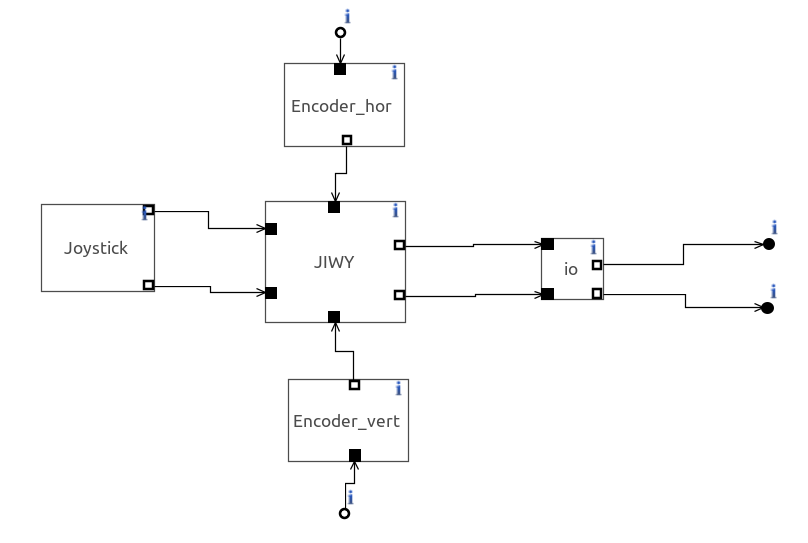
\includegraphics[width=0.7\textwidth]{./img/jiwy-overview.png}
	\caption{Top architecture model of the Ex2 JIWY model.}
	\label{fig:jiwy-overview}
\end{figure}
\subsubsection{Joystick input handling.}
This model (figure~\ref{fig:jiwy-joystick}) contains \cpp code blocks that implement the Joystick 
functionality as suggested in Appendix B of the assignment document.

\begin{figure}[ht]
	\centering
	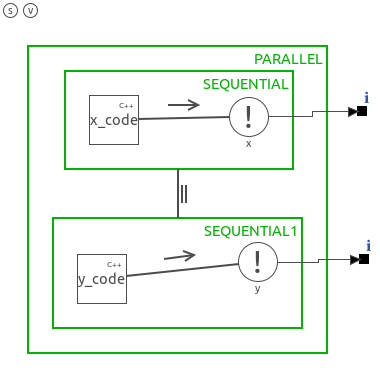
\includegraphics[width=0.4\textwidth]{./img/jiwy-joystick.png}
	\caption{The JIWY Joystick submodel}
	\label{fig:jiwy-joystick}
\end{figure}
See codeblock~\ref{code:x_code} for relevant code of the \texttt{x\_code} codeblock. \texttt{y\_code} is almost identical.

\begin{lstlisting}[caption=x\_code Joystick C++ code block, label=code:x_code, language=C++]
/**
 * Source file for the x_code model
 * Generated by the TERRA CSPm2LUNA generator version 1.1.3
 *
 * protected region document description on begin
 *
 * protected region document description end
 */

#include "x_code.h"
// protected region additional headers on begin
// Each additional header should get a corresponding dependency in the Makefile
#include "hid/HID.h"
#include "csp/Reader.h"
#include "string.h"
// protected region additional headers end

namespace Joystick { namespace x_code { 

x_code::x_code(double &x) :
    CodeBlock(), x(x){
  SETNAME(this, "x_code");

  // protected region constructor on begin
  channel = new LUNA::CSP::HIDAbsAxisChannel("/dev/joystick2", 1);
  reader = new LUNA::CSP::Reader<double>(&x,channel);

  buttonchannel = new HIDButtonChannel("/dev/joystick2", 1);
  buttonreader = new LUNA::CSP::Reader<bool>(&btn,buttonchannel);

  // protected region constructor end
}

x_code::~x_code()
{
  // protected region destructor on begin
	delete channel;
	delete reader;
	delete buttonreader;
  // protected region destructor end
}

void x_code::execute()
{
  // protected region execute code on begin
	channel->read(reader);
	buttonchannel->read(buttonreader);
	// scale
	this->x = (x - 512.0)/-512.0;

	//printf("Joystick_x: i read %f\n", x);

	if (btn)
		{
			printf("Smile!!!\n");
			std::terminate();
		}
  // protected region execute code end
}

// protected region additional functions on begin
// protected region additional functions end
// Close namespace(s)
} } 
\end{lstlisting}
\subsubsection{JIWY model.}
The overview model's (figure~\ref{fig:jiwy-overview}) JIWY model (figure~\ref{fig:jiwy-jiwy}) 
is very similar to the model we looked at in exercise 1. The only difference is that 
It has imported models from the given 20sim JIWY model, 'Horizontal' and 'Vertical'.
\begin{figure}[ht]
	\centering
		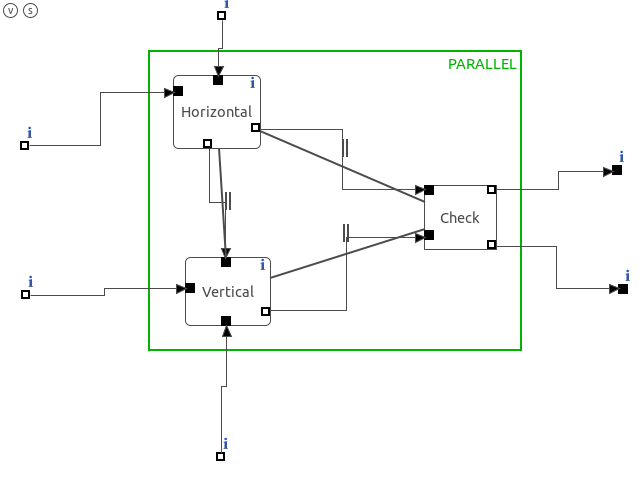
\includegraphics[width=0.6\textwidth]{./img/jiwy-jiwy.png}
		\caption{JIWY}
		\label{fig:jiwy-jiwy}
\end{figure}

See figure~\ref{fig:jiwysubmodel} for the submodels of Horizontal, Vertical and Check.
\subsubsection{IO output handling.}
The IO model of our top-level model (figure~\ref{fig:jiwy-overview}) converts input from JIWY (double) to HW port (\texttt{uint16\_t}). See figure~\ref{fig:jiwy-IO}.
Codeblock~\ref{code:IO} presents the relevant code that is used to do the conversion.
Note that the code of \texttt{hor\_convert} and \texttt{ver\_convert} is identical.
\begin{figure}[ht]
	\centering
	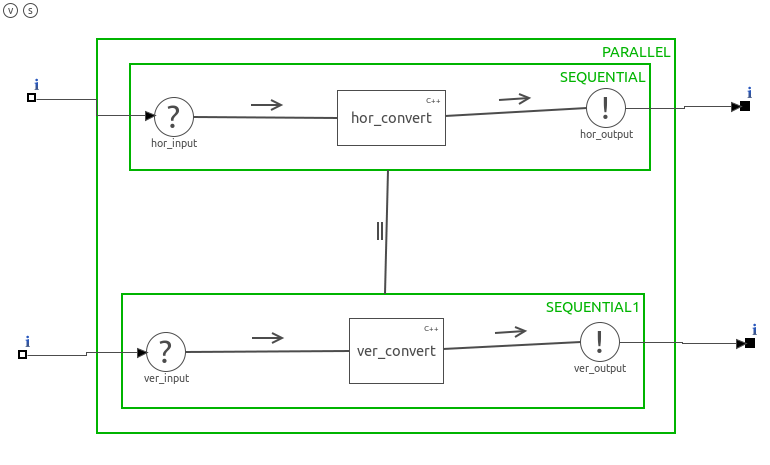
\includegraphics[width=0.7\textwidth]{./img/jiwy-IO.png}
	\caption{IO}
	\label{fig:jiwy-IO}
\end{figure}
\begin{lstlisting}[caption=Relevant code of the IO block, label=code:IO, language=C++]
void ver_convert::execute()
{
  // protected region execute code on begin
	this->ver_output = convert(this->ver_input);
	printf("Vertical: in: %f, out: %d\n", ver_input, ver_output);
  // protected region execute code end
}

// protected region additional functions on begin
uint16_t ver_convert::convert(double f)
{
	int16_t deadzone = 1000;

	int16_t n = f*(32768-deadzone);
	if(n>0)
		n += deadzone;
	else if(n<0)
		n -= deadzone;

	return (uint16_t)n;
}
\end{lstlisting}

\subsubsection{Vertical and Horizonal encoding handling.}
\texttt{Encoder\_hor} and \texttt{Encoder\_vert} of the top-level model (figure~\ref{fig:jiwy-overview}) are very similar. They both consist of a \cpp codeblock that does some conversion. 
Specifically, converting from \texttt{uint32\_t} to \texttt{double}. 

See figure~\ref{fig:jiwy-encoder} for a screenshot of the encoder model, and 
codeblock~\ref{code:encoder} for the code (same code in \texttt{Encoder\_Hor} and \texttt{Encoder\_vert}).
\begin{figure}[ht]
	\centering
	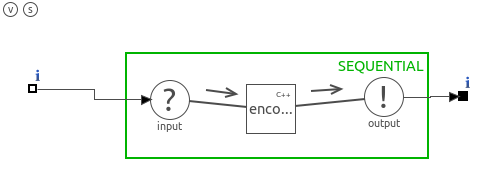
\includegraphics[width=0.7\textwidth]{./img/jiwy-encoder.png}
	\caption{Encoder}
	\label{fig:jiwy-encoder}
\end{figure}
\begin{lstlisting}[caption=Relevant code of the Encoder\_vert and Encoder\_hor models, label=code:encoder, language=C++]
void encodervert::execute()
{
  // protected region execute code on begin
	this->output = scale(convert(this->input));
	printf("%f\n", this->output);
  // protected region execute code end
}

// protected region additional functions on begin
double encodervert::convert(uint32_t i)
{
	return (int32_t)i;
}

double encodervert::scale(double n)
{
	return (n/6000)*2*M_PI;
}
\end{lstlisting}
\subsection{Test at the lab}
During the lab test we had a few problems. However, we got it working in the end.

Here is a list of things that we had to adjust in the lab:
\begin{itemize}
	\item Joystick input was not working: when creating the \texttt{HIDAbsAxisChannel} we entered an arbitrary string instead of the `/dev/joystick2' device file.
	\item The output of our Joystick component was not normalized to $-1$ .. $1$.

		We understood from the 20sim model that the JIWY controller model input was a value between $-512$ and $512$, this is wrong.
	\item The IO sub-module's \cpp codeblocks had their variables erroneously linked with the wrong parent variables.
	\item The Joystick input was reversed, so we multiplied it by $-1$.
	\item The conversion code of the IO block was initially in the check part of the JIWY model.
		We changed this to a separate model because it makes more sense. The conversion to \texttt{uint16\_t} has nothing to do with the JIWY model.
	\item The JIWY model expected radian values for the angles of the motors. We had to do some scaling to achieve this.
	\item The JIWY model output for PWM ranged from $-1$ to $1$, not from $-512$ to $512$ as we initially thought. This was easily fixed.
	\item JIWY had trouble keeping the camera still when we mapped every non-zero value to a PWM value outside the deadzone. So we re\"introduced a deadzone, slightly smaller than the original one, by assuming a deadzone between $-1000$ and $1000$, instead of $-2200$ and $2200$. This maps small values to within the actual deadzone of the motor.
\end{itemize}

\subsection{Questions}
\begin{enumerate}
	\item We put scaling code in two models called \texttt{Encoder\_hor} and 
		\texttt{Encoder\_vert}. See figure~\ref{fig:jiwy-overview} and codeblock~\ref{code:encoder} for the code.
		
		We put scaling code in the Joystick submodel, see codeblock~\ref{code:x_code} line $49$.
		
		We put scaling code in the IO submodel, see codeblock~\ref{code:IO}

		We put the scaling code models outside of the JIWY model because we see it as an extra layer to the JIWY model, instead of a part of the JIWY model itself.
	\item This is best implemented inside the check JIWY submodel, shown in figure~\ref{fig:jiwysubmodel-check}, as a layer between the JIWY calculation, and the actual IO conversion.
\end{enumerate}

\subsection{Further functionality}
We implemented joystick button functionality and a way to exit the program without CTRL-C.

\subsection{Questions}
\begin{enumerate}
	\item Not applicable
	\item Moving parts could by obstructed by, in the worst case, bodyparts. In this case, the motors are not powerful enough to really inflict damage on its surrounding, but it could damage its own motors or mechanics by hitting obstructions. When the software detects unexpected values from its sensors, signalling that the hardware is not doing what it should do, all moving parts could be stopped to prevent damage. This is best implemented in a similar place as the check for hitting endstops.
	
	Another possibility is misfunctioning sensors, giving a static signal or a very noisy one. This would make it impossible for JIWY to function properly. To implement this, the faulty behaviour needs to be detected. This should be done by comparing the actual sensor data to the expected values. If the actual data is very different from the expected values, the process should switch to another mode (simplest would be just to stop). This needs an adjustment in the 20-sim model, to generate expected sensor values, and then CSP submodel need to be added to compare expected values with the actual values.
	
	\item We could hold the camera, keeping it from moving to test how the system deals with physical obstructions. We could simulate faulty sensor data to test the fault detected, or actually break the sensors. This last option is of course not desirable.
	
	\item See figure~\ref{fig:slide}. The exercises on JIWY started with a given CSP model that was mostly filled in and that had to be checked for deadlocks/livelocks (exercise 1.4.x). This part corresponds to 1b and 2b. Part 2c (Control laws) is given in this exercise set, it is the 20sim model of the JIWY controller in exercise 2. Part 3a corresponds with the work in exercise 2 that was done at home: the generation of TERRA CSP models of the given 20sim model, the addition of Joystick input and adding encoder/PWM ports. The simulations done at home correspond to step 3b. Lastly, the exercise in the lab corresponds to step 4.

	The parts of the design flow that are related to the plant dynamics modeling did not appear in the  JIWY exercise set, they were given. This is, presumably, because the course is focused on the software development of real-time embedded systems. 
\end{enumerate}

\begin{figure}[ht]
	\centering
	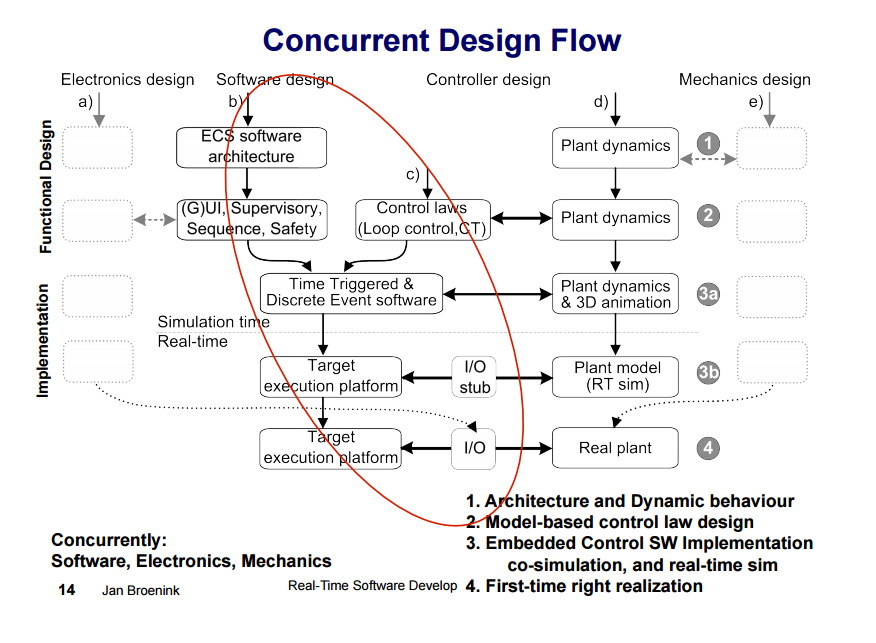
\includegraphics[width=0.7\textwidth]{./img/slide.png}
	\caption{061-Law-Code.pptx.pdf slide 14}
	\label{fig:slide}
\end{figure}

\begin{figure}[ht]
	\begin{subfigure}{\textwidth}
		\centering
		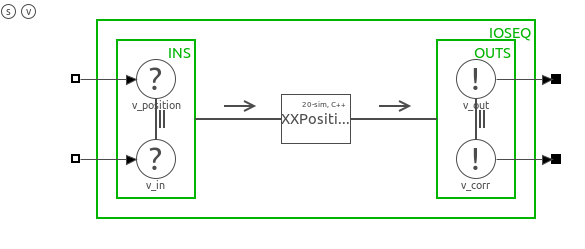
\includegraphics[width=0.8\textwidth]{./img/jiwy-jiwy-hor.png}
		\caption{Horizonal}
	\end{subfigure}
	\begin{subfigure}{\textwidth}
		\centering
		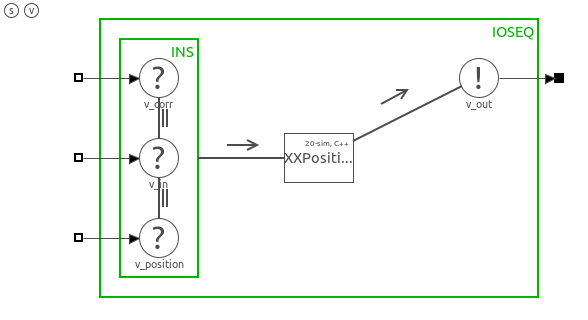
\includegraphics[width=0.7\textwidth]{./img/jiwy-jiwy-ver.png}
		\caption{Vertical}
	\end{subfigure}
	\begin{subfigure}{\textwidth}
		\centering
		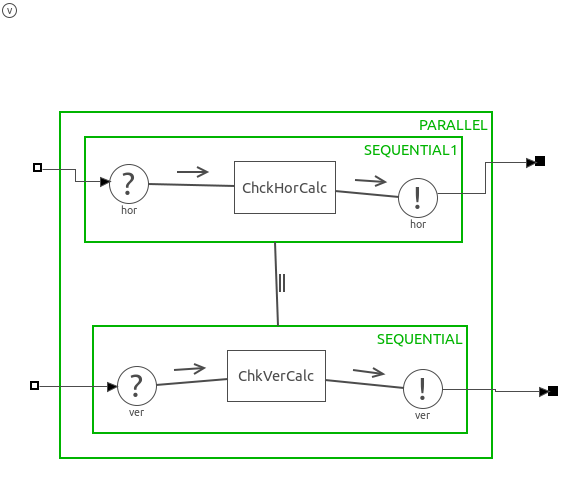
\includegraphics[width=0.7\textwidth]{./img/jiwy-jiwy-check.png}
		\caption{Check}
		\label{fig:jiwysubmodel-check}
	\end{subfigure}
	\caption{JIWY submodels.}
	\label{fig:jiwysubmodel}
\end{figure}


\end{document}
